\documentclass[12pt,aspectratio=169,notheorems]{beamer}
\graphicspath{
	{img}
}

\usetheme[progressbar=frametitle, numbering=fraction]{metropolis}
\usepackage{appendixnumberbeamer}
\usepackage[font=small,labelfont=bf]{caption}
\usepackage{hyperref}

\setbeamercolor{background canvas}{bg=white}

\usepackage{booktabs}
\usepackage[scale=2]{ccicons}

% Change Color of the theme
\usepackage{xcolor}
\definecolor{DarkGrey}{HTML}{353535}
\definecolor{ECNURed}{RGB}{164,31,53}
\definecolor{ECNUBrown}{RGB}{134,117,77}
\setbeamercolor{normal text}{ fg= DarkGrey  }
\setbeamercolor{alerted text}{ fg= ECNURed  }
\setbeamercolor{example text}{ fg= ECNUBrown  }



\title{\LARGE AI Project Report}
\subtitle{Network Intrusion Detection System}
\author{\\ Andrea Mugnai \\ Jacopo Tucci}
\date{2024/2025}
\titlegraphic{\hfill
\includegraphics[height=2cm]{logo.png}}

\begin{document}

\maketitle

\begin{frame}{Goals}
    Our goal is to create a Network Intrusion Detection System (NIDS) capable of classifying raw network packets into the following categories:
    \begin{itemize}
        \item Normal
        \item Denial of Service (DoS)
        \item User to Root (U2R)
        \item Remote to Local (R2L)
        \item Probe
    \end{itemize}
    The classification models used for this task are based on \textbf{supervised learning}.
\end{frame}

\begin{frame}{Dataset}
    We used a non cleaned dataset: \href{https://research.unsw.edu.au/projects/unsw-nb15-dataset}{UNSW-NB15}. 
    The raw packet was created by the \texttt{IXIA PerfectStorm tool}. This dataset is a labeled datset and in particular has nine types of attacks 
    that we mapped in the categories we mentioned before as follows:
    \begin{itemize}
        \item DoS: DoS, Worms.
        \item U2R: Backdoor, Shellcode.
        \item R2L: Exploits, Analysis.
        \item Probe: Reconnaissance, Fuzzers, Generic.
        \item Normal: Benign packets.
    \end{itemize}
        \small We used the \texttt{label} column to map the attacks to categories. In particular all the \texttt{attack\_cat} values were empty for the \texttt{Normal} class. \\
\end{frame}

\begin{frame}{Category Distribution}
        \footnotesize The dataset is highly unbalanced, with the majority of the samples belonging to the \textbf{Normal} class.
    \begin{center}
        \hspace*{-0.8cm}
        \begin{minipage}[t][6cm][t]{0.5\textwidth}
            \centering
            \vspace{-0.08cm}
            \fbox{ % Adds a border around the table
                \resizebox{1.2\textwidth}{!}{%
                    \begin{tabular}{|l|l|l|l|l|l|l|l|l|l|}
                        \hline
                        \textbf{Normal} & \textbf{Generic} & \textbf{Exploits} & \textbf{Fuzzers} & \textbf{Reconnaissance} & \textbf{DoS} & \textbf{Backdoor} & \textbf{Analysis} & \textbf{Shellcode} & \textbf{Worms} \\
                        \hline
                        281,462 & 6,894 & 6,851 & 4,970 & 3,420 & 1,465 & 623 & 621 & 371 & 42 \\
                        \hline
                    \end{tabular}
                }
            }
            \caption{Counts for each attack category.}
            \label{tab:inverted_attack_categories}

            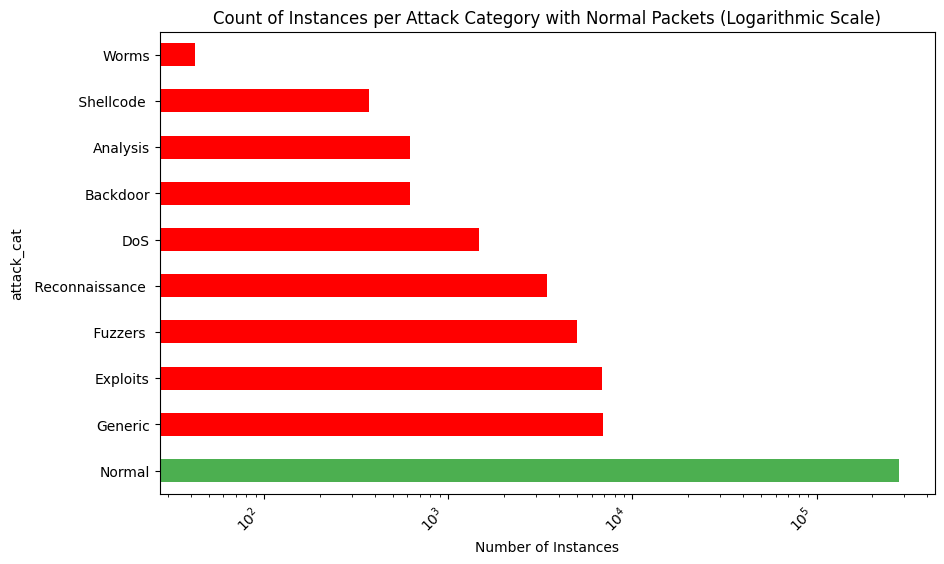
\includegraphics[width=\textwidth, height=5cm, keepaspectratio]{attack_cat_before.png} \\
            \textit{Original Dataset \emph{attack category} distribution}
        \end{minipage} 
        \hfill
        \begin{minipage}[t]{0.45\textwidth}
            \centering
            \vspace{-0.01cm}
            \fbox{ % Adds a border around the table
                \resizebox{0.7\textwidth}{!}{%
                    \begin{tabular}{|l|l|l|l|l|l|}
                        \hline
                        \textbf{Normal} & \textbf{Probe} & \textbf{R2L} & \textbf{DoS} & \textbf{U2R} \\
                        \hline
                        281,462 & 15,284 & 7,472 & 1,507 & 994 \\
                        \hline
                    \end{tabular}
                }
            }
            \caption{Counts for each attack category.}
            \label{tab:inverted_attack_categories}
            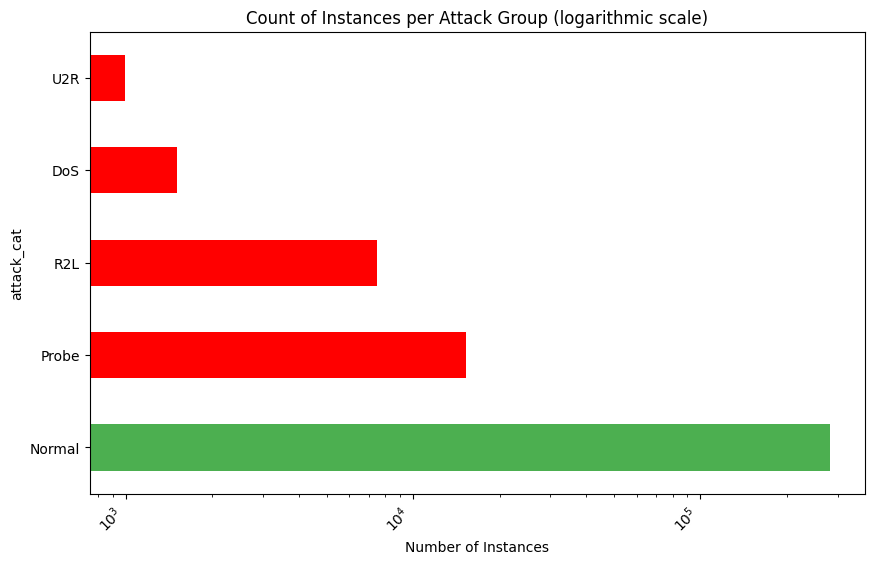
\includegraphics[width=\textwidth, height=4.5cm, keepaspectratio]{attack_cat_after.png} \\
            \textit{Our Dataset \emph{attack category} distribution}
            
        \end{minipage}
        \hspace*{-1cm}
        
    \end{center}
\end{frame}

\begin{frame}{Identify Missing and Erroneus Values }
        \scriptsize 
        We identified 49 features in the dataset, 42 of which are numerical and 7 are categorical.
        The Dataset contained missing values: 
        \begin{table}[]
            \centering
            \resizebox{0.5\textwidth}{!}{%
                \begin{tabular}{|l|l|l|l|l|}
                \hline
                               & ct\_flw\_http\_mthd & is\_ftp\_login & service & ct\_ftp\_cmd\\ \hline
                Missing Values & 273700              & 300350         & 167857 & 300350 \\ \hline
                \end{tabular}%
            }
        \end{table}        
        The \emph{attributes }\texttt{ct\_flw\_http\_mthd} indicates how many \emph{HTTP} method are present is correlated with 
        the value \textt{http} in \texttt{service} but we found a discrepancy:
        \begin{table}[]
            \centering
            \resizebox{0.4\textwidth}{!}{%
                \begin{tabular}{|l|l|l|l|}
                \hline
                               & ct\_flw\_http\_mthd & service 'http' \\ \hline
                Count Values & 33019             & 32777  \\ \hline
                \end{tabular}%
            }
        \end{table}
        This means that the differences '242' that are signed as missing in \texttt{service} can be set to \texttt{http}.  \\
        \vspace{2ex}
        Analysing the attributes \texttt{is\_ftp\_login}, \texttt{ct\_ftp\_cmd} we notice that they are equals in number, in values and in raws.  
        Probably one of them is wrong, even if not anyway the attributes together are redundant.
\end{frame}

\begin{frame}{Architecture}
    \begin{center}
        \includegraphics[scale=.65]{architecture-v1.png}
    \end{center}
\end{frame}

\begin{frame}{Database - ER diagram details}
    The \emph{N-to-N} relationship between \textbf{Player} and \textbf{Gacha} will be implemented with the table \textbf{Player\_Gacha}. The \textbf{Player\_Auction} table expresses the \emph{N-to-N} relationship between \textbf{Player} and \textbf{Auction}. When a player wins an auction and pays the gacha, a transaction record will be created. \\[1ex]
    Each auction is created by one player (i.e. \emph{create} relationship) and it will contain a reference to a transaction record when the winning player pays the bid. For \textbf{Transaction} records, we store the creation datetime. \\[1ex]
    The gacha's rarities are stored inside \textbf{Rarity} table and each gacha maintains a reference to a specific rarity.
\end{frame}

\begin{frame}{User's interactions}
      A player can do a bid only if he has enough currency. The payment operation will be done automatically by the system at the end of the auction. If he cannot pay (e.g. due to no found), the runner-up player will become the winner. \\[1ex]
     We consider in-coming transactions (i.e. player sells a gacha) and out-going ones (i.e. player buys a gacha). In the OpenAPI specifications, we use \textbf{from} and \textbf{to} attributes to distinguish between them.
\end{frame}

\end{document}
